\chapter{Validation par comparaison avec l'expérience}
L'objectif de cette partie est de comparer les résultats obtenus via TrioCFD et l'utilisation d'une description analytique de l'énergie avec ceux présentés par Rao et al. \cite{rao_influence_2015}. Dans leur article Rao et al. présentent une expérience ainsi qu'un modèle CFD associé à l'experience permettant de modéliser le transfert de masse pour un cas ternaire.
\section{Présentation du cas de référence}
L'objectif de l'expérience présenté par Rao et al. est de visualiser, au travers d'une expérience, la diffusion massique d'une goutte composée d'acétonitrile (miscible dans l'eau) et de chlorobenzène (immiscible) dans de l'eau. A l'instant initial la goutte formée a une masse volumique inférieure à celle de l'eau créant un mouvement ascendant de la goutte, puis sous l'effet de la diffusion de l'acétonitrile la densité de la goutte va augmenter et la goutte va redescendre. Le schéma de l'installation expérimentale est présenté ci-dessous :
\begin{figure}[H]
	\centering
	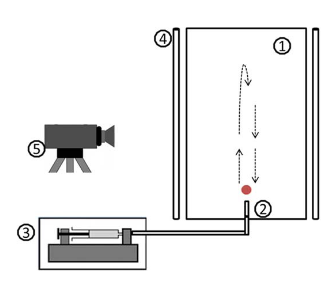
\includegraphics[width=0.3\linewidth]{figure/exp}
	\caption{Schéma de l'installation expérimentale, d'après \cite{rao_influence_2015}}
	\label{fig:exp}
\end{figure}
L'article présente également un modèle CFD, dans celui-ci le transfert de masse est calculé semi-empiriquement, à chaque itération la position de la goutte obtenue numériquement est comparée à la position obtenue expérimentalement, puis une régulation est mise en place pour déterminer un coefficient de transfert de masse via des corrélations pour faire diminuer cet écart, le ”modèle” alors obtenu n’est pas prédictible et une expérience physique est toujours nécessaire pour réaliser une simulation. L'algorithme est présenté en figure \ref{fig:algoRao}, 
\begin{figure}[H]
	\centering
	\begin{tikzpicture}[scale=0.75, transform shape]
	\node[draw,aspect=1.3, text centered,text width=3cm] (V) at (0,2.3) {Solution initiale };
	\node[draw,aspect=1.3, text centered,text width=2cm] (T) at (0,1.3) {$n=n+1$ };
	\node[draw,rectangle, text centered,minimum width=2cm,minimum height=1cm] (A)at(0,0){Estimation du transfert de masse à partir de corrélations};
	\node[draw,text centered,minimum width=2cm,minimum height=1cm] (B) at (0,-1.5) {Résolution des équations de Navier-Stokes};
	\node[draw,text centered,text width=10cm,minimum height=1cm] (C) at (0,-3) {Comparaison entre l'altitude de la goutte obtenue par CFD avec l'expérience, res = $f(z_{\text{CFD}},z_{\text{exp}})$};
	\node[draw,rectangle,diamond, aspect=1.3, text centered,text width=1.5cm] (D) at (0,-5) {res $<\varepsilon$ ? };
	
	\node[draw,rectangle,diamond, aspect=1.3, text centered,text width=1.5cm] (E) at (0,-7.3
	) { $t^{f}<t^{n}$ ? };
	\node[draw,aspect=1.3, text centered,text width=1.5cm] (W) at (0,-9) {Fin};
	%\node[draw,text centered,text width=2cm,minimum height=1cm] (E) at (0,-6.8) { $t=t^{n+1}$};
	%\node[draw,text centered,text width=7cm,minimum height=1cm] (Z) at (0,-6.2) { dsq}
	
	\node[draw,rectangle,diamond, aspect=1.3, text centered,text width=1cm,color=white] (H)at(-5,-5.9){ };
	\node[text centered,text width=1cm,color=black] (K1)at(0.5,-5.9){oui};
	\node[text centered,text width=1cm,color=black] (K2)at(-1.5,-4.8){non};
	\node[text centered,text width=1cm,color=black] (K3)at(0.5,-8.3){oui};
	\node[text centered,text width=1cm,color=black] (K4)at(-1.5,-7){non};
	%\node[draw,rectangle, text centered,diamond, aspect=1.3, text centered,text width=1cm] (I)at(6,-6){i=1 to n-1};
	\draw[->] (T.south) -- (A.north);
	\draw[->] (A.south) -- (B.north);
	\draw[->] (B.south) -- (C.north);
	\draw[->] (C.south) -- (D.north);
	\draw[->] (D.south) -- (E.north);
	\draw[->] (V.south) -- (T.north);
	\draw[->] (E.south) -- (W.north);
	\draw[->] (-7,1.3) -- (T.west);
	
	
	
	\draw (D.west)-- (-6,-5);
	\draw (-6,-5)-- (-6.,0);
	%	\draw (F.west)-- (-6.,0);
	\draw[->] (-6.,0) -- (A.west);
	\draw[-] (E.west) -- (-7,-7.3);
	\draw[-] (-7,-7.3) -- (-7,1.3);
	%\draw (G.east)-| (I.south);
	%\draw[->] (I.north)|- (A.east);
	\end{tikzpicture}
	\caption{Algorithme de résolution développé par Rao et al.\cite{rao_influence_2015}}
	\label{fig:algoRao}
\end{figure}
\section{Critères graphique de choix du paysage thermodynamique}
Dans cette partie les critères graphiques de choix du paysage thermodynamique seront présentés, ces critères permettent de savoir si un paysage est potentiellement cohérent avec le système étudié.
Dans un premier temps il est essentiel que les conditions initiales ne soient pas incluse dans la lacune de miscibilité, ce qui entraînerait une séparation de phase immédiate, un exemple de ce type est donnée en figure \ref{fig:landscapebase} et les résultats sont présentés par la figure \ref{land_base_sep}, on y observe une séparation de phase dès les premiers instants du calcul avec la présence de deux phases à l'intérieur de la goutte, une première uniquement composée de l'élément immiscible et la seconde composée d'eau et de l'élément miscible.
 \begin{figure}[H]
 	\centering
 	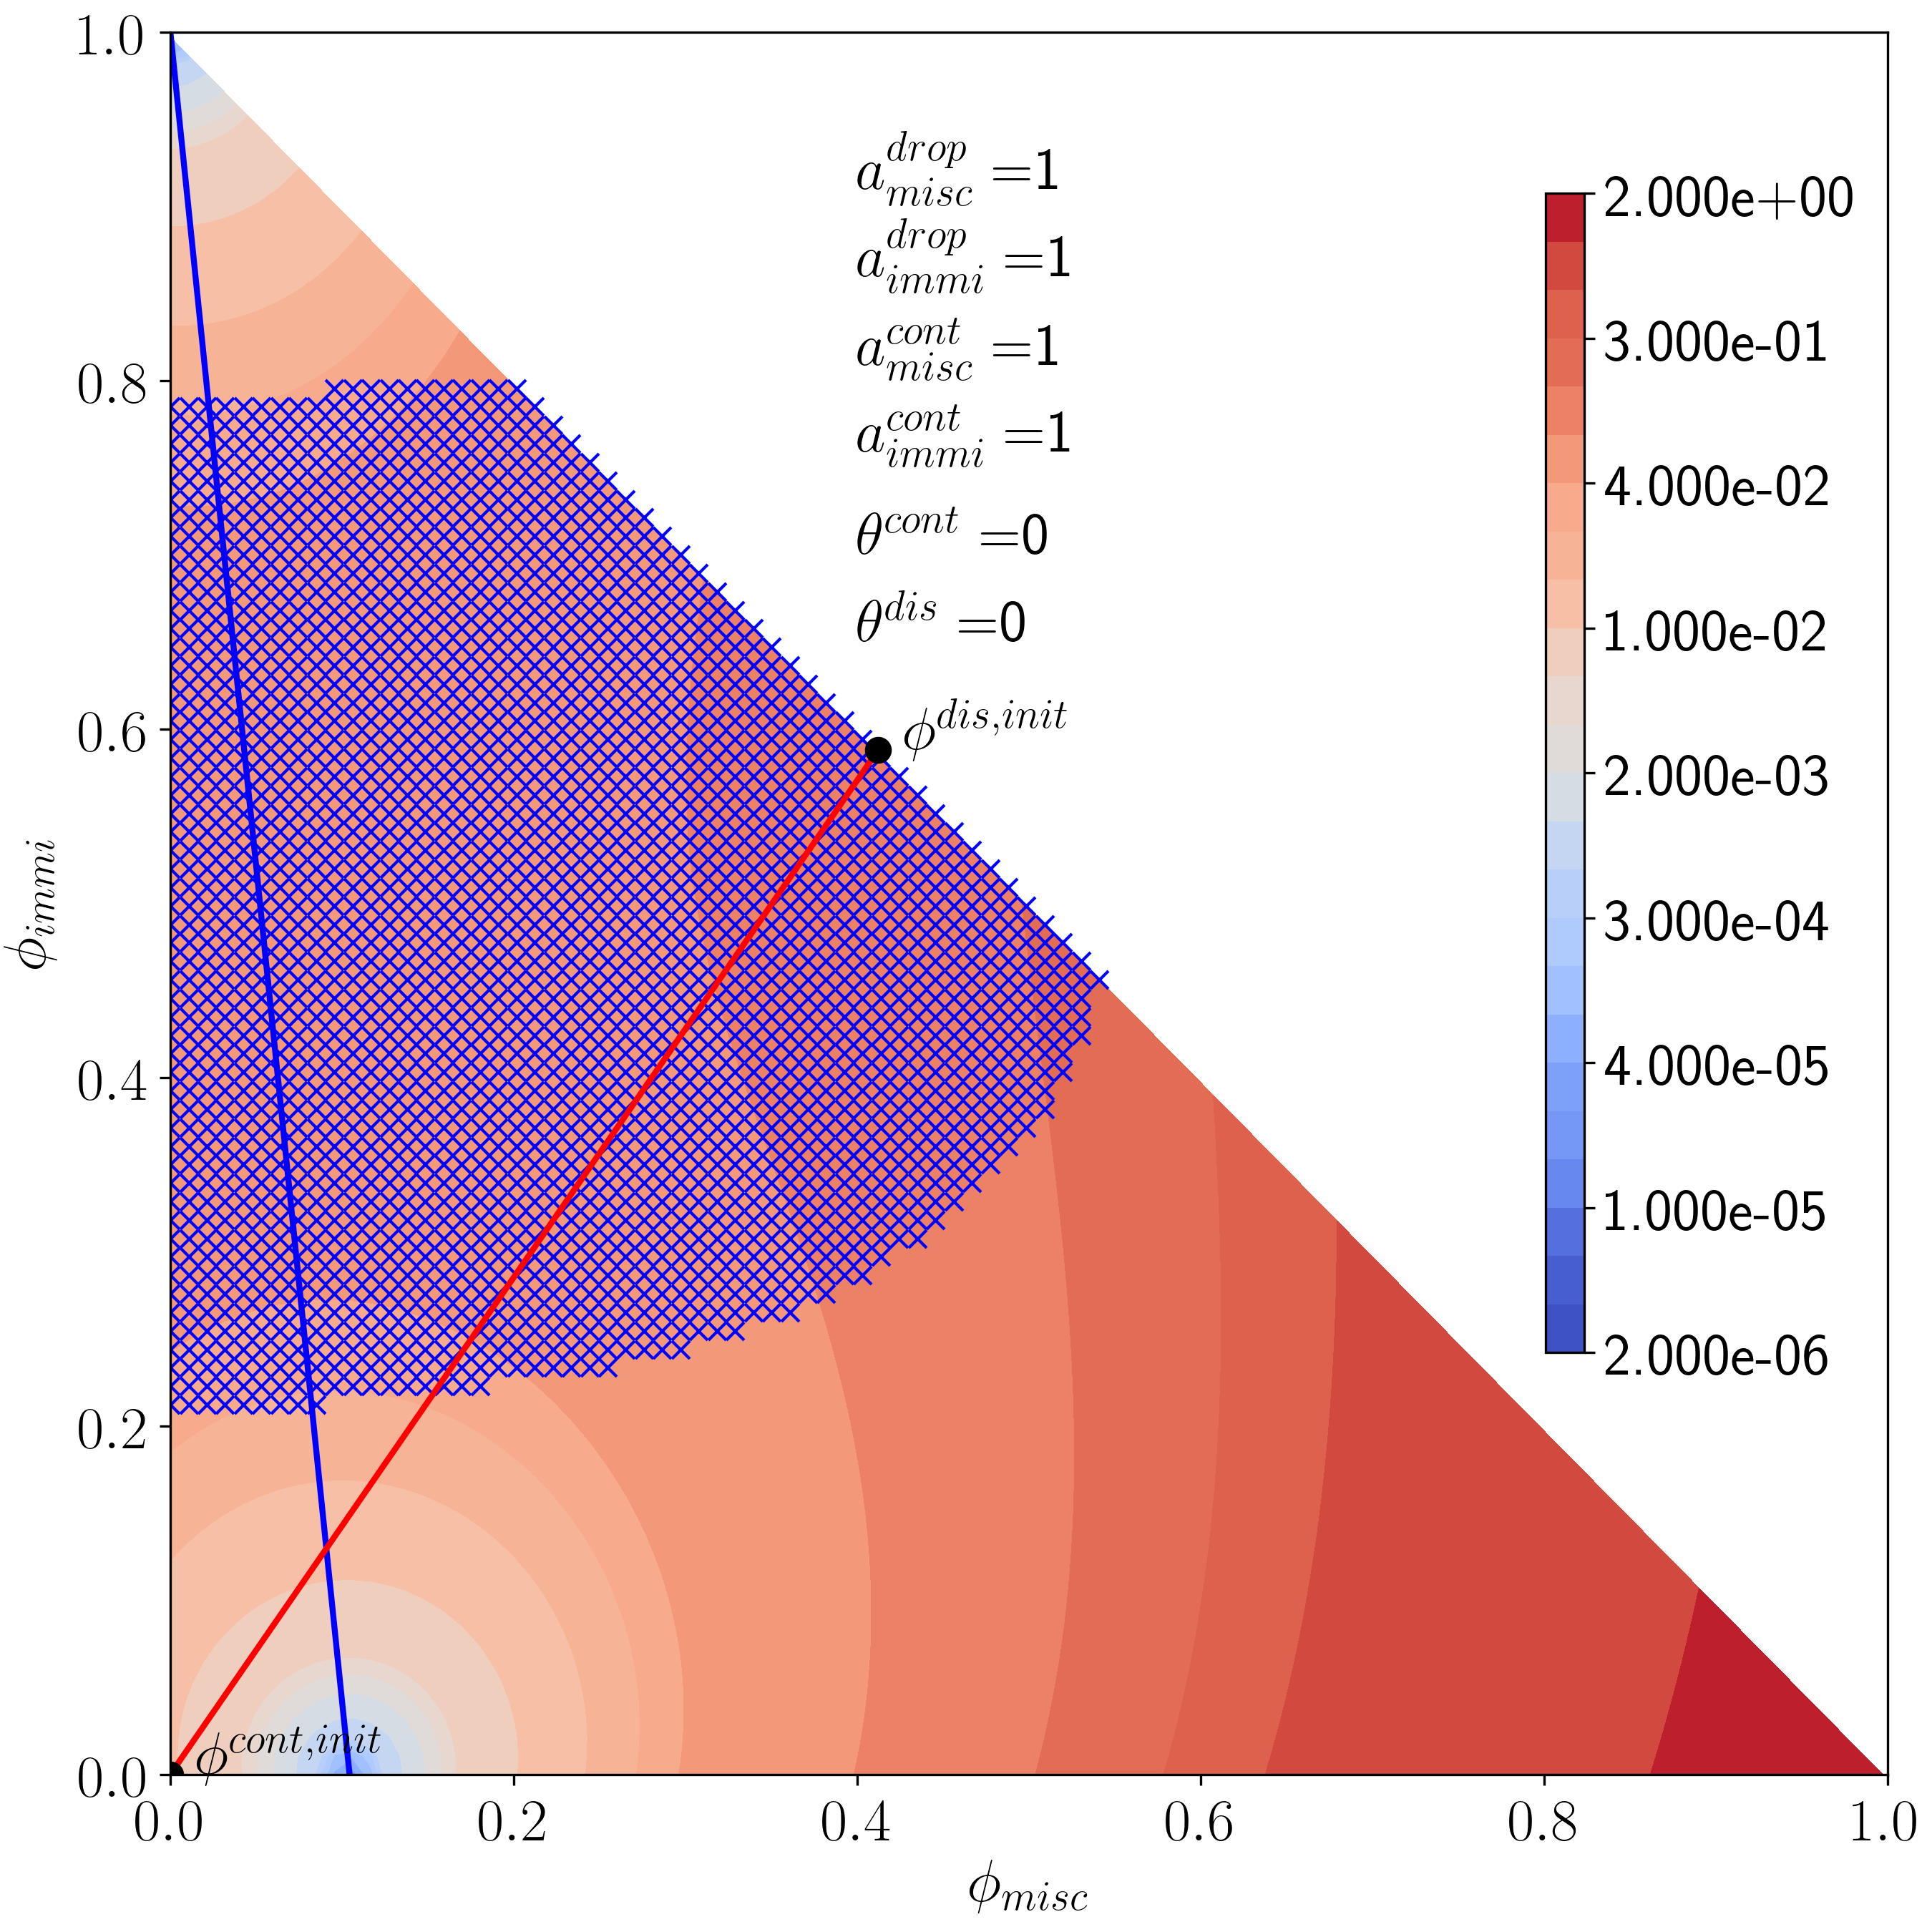
\includegraphics[width=0.4\linewidth]{figure/landscape_base.png}
 	\caption[Paysage thermodynamique]{Paysage thermodynamique, la droite bleu relie les deux  concentrations d'équilibre, la droite rouge relie les deux concentrations initiales}
 	\label{fig:landscapebase}
 \end{figure}
\vspace{-0.5cm}
 \begin{figure}[H]
 	\centering
 	\begin{subfigure}[H]{0.32\textwidth}
 		\centering
 		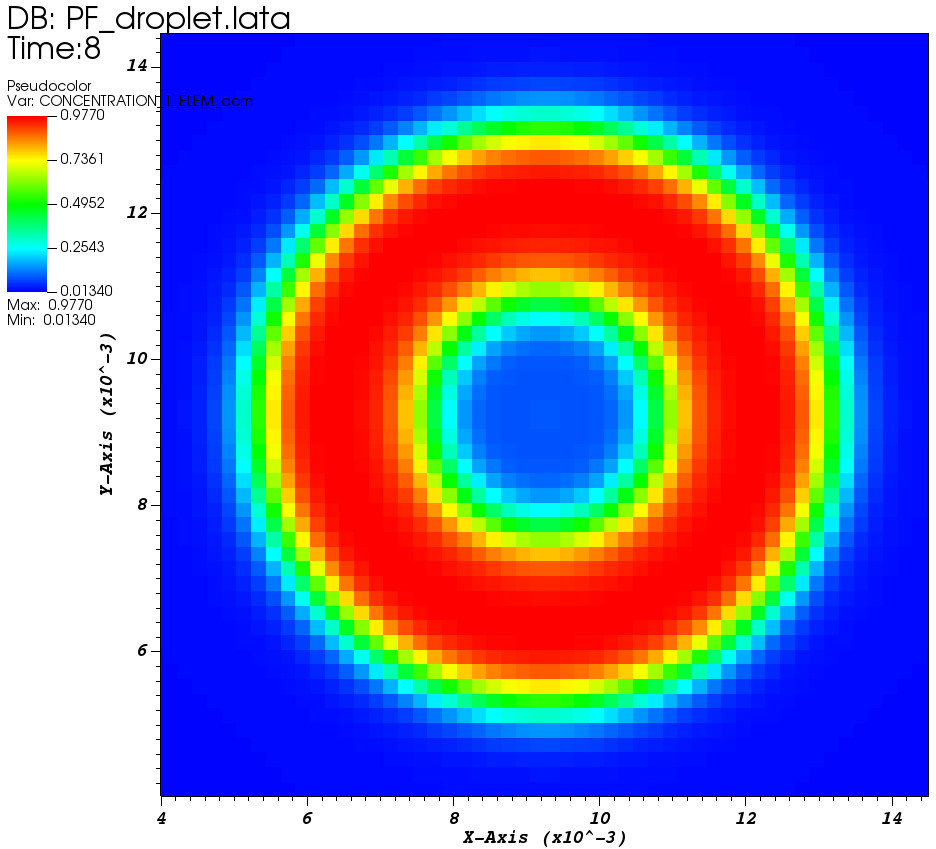
\includegraphics[width=\textwidth]{figure/paysage_base/visit0000.png}
 		\caption{Concentration immiscible}
 		\label{fig:y equals x}
 	\end{subfigure}
 	\begin{subfigure}[H]{0.32\textwidth}
 		\centering
 		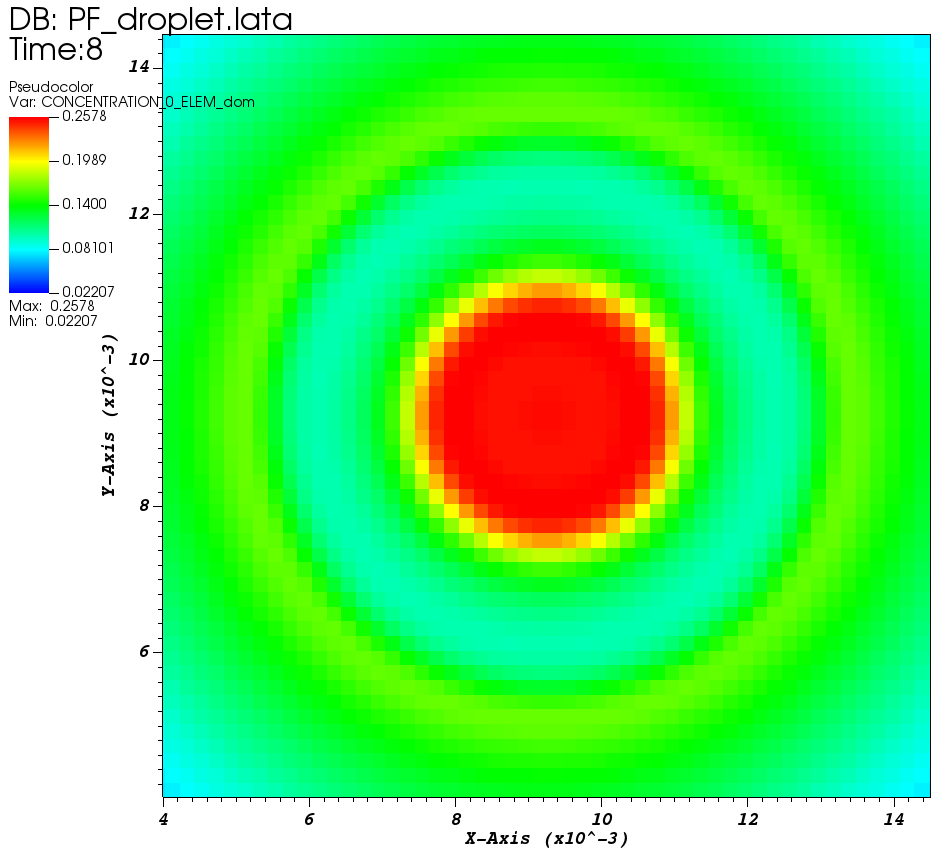
\includegraphics[width=\textwidth]{figure/paysage_base/visit0001.png}
 		\caption{Concentration miscible}
 		\label{fig:y equals x}
 	\end{subfigure}
 	\begin{subfigure}[H]{0.32\textwidth}
 		\centering
 		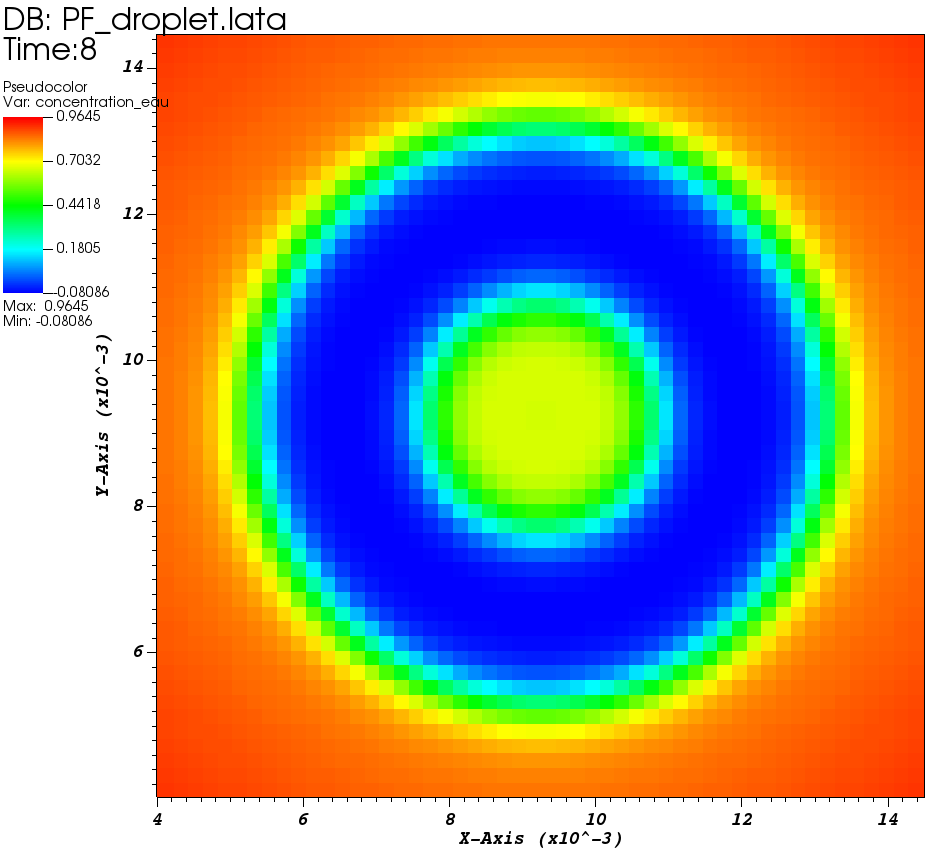
\includegraphics[width=\textwidth]{figure/paysage_base/visit0002.png}
 		\caption{Concentration eau}
 		\label{fig:y equals x}
 	\end{subfigure}
 	\caption{Séparation de phase dans la goutte}
 	\label{land_base_sep}
 \end{figure} \vspace{-0.5cm}

Le deuxième critère concerne la direction privilégiée par le système, on présente un deuxième paysage en figure \ref{fig:paysage2}. En effet l'objectif est également de limiter l'entrée d'eau dans la goutte, pour cela il est nécessaire qu'en tout point de la goutte la somme des compositions des composants miscible et immiscible soit égale à l'unité. Pour que cela soit toujours le cas il est important que l'orientation des gradients soit favorable dès l'instant initial. La figure \ref{fig:gradpasbon} présente un exemple où ce gradient favorise une entrée d'eau dès les premiers instants, dans cette exemple le gradient favorise également un chemin qui passe par la zone instable, ainsi on peut également prévoir une séparation de phase, l'ensemble de ces phénomène peuvent être observés sur la figure \ref{fig:eauref}, l'entrée d'eau dès les premiers instants (t$=0.3$s) puis la séparation de phase (t$=10$s et t$=25$s) pour finalement retrouver l'état stationnaire attendu d'une goutte homogène ne contenant pas d'eau aux temps long (t$=50s$).

%Comme expliqué précédemment ce paysage représente l'énergie libre volumique liée à l'équilibre des phases, ainsi on cherche à ce que les conditions initiales (ici aux extrémités de la droite rouge) soit hors de la zone instable et que la composition d'équilibre globale (placé a l'intersection des droites bleu et rouge) soit placée dans la lacune de miscibilité. Ainsi ce paysage semble correspondre parfaitement à ces deux critères. On souhaite également limiter l'entrée d'eau dans la goutte en régime transitoire, cette condition ce traduit par égalité entre la somme des deux compositions et l'unité. Hors ici le gradient d'énergie favorise un "chemin" différent. Pour vérifier cette présence d'eau, on considère alors un calcul statique (sans résolution des équations de Navier-Stokes) et on trace les concentrations à différents instants. On observe dès lors une importante intrusion d'eau dans la goutte dès les premiers instants, puis une séparation de phase est observable à l'intérieur de la goutte, phénomène que l'on souhaite absolument éviter.
 \begin{figure}[H]
 	\centering
 	\begin{subfigure}[H]{0.45\textwidth}
 		\centering
 		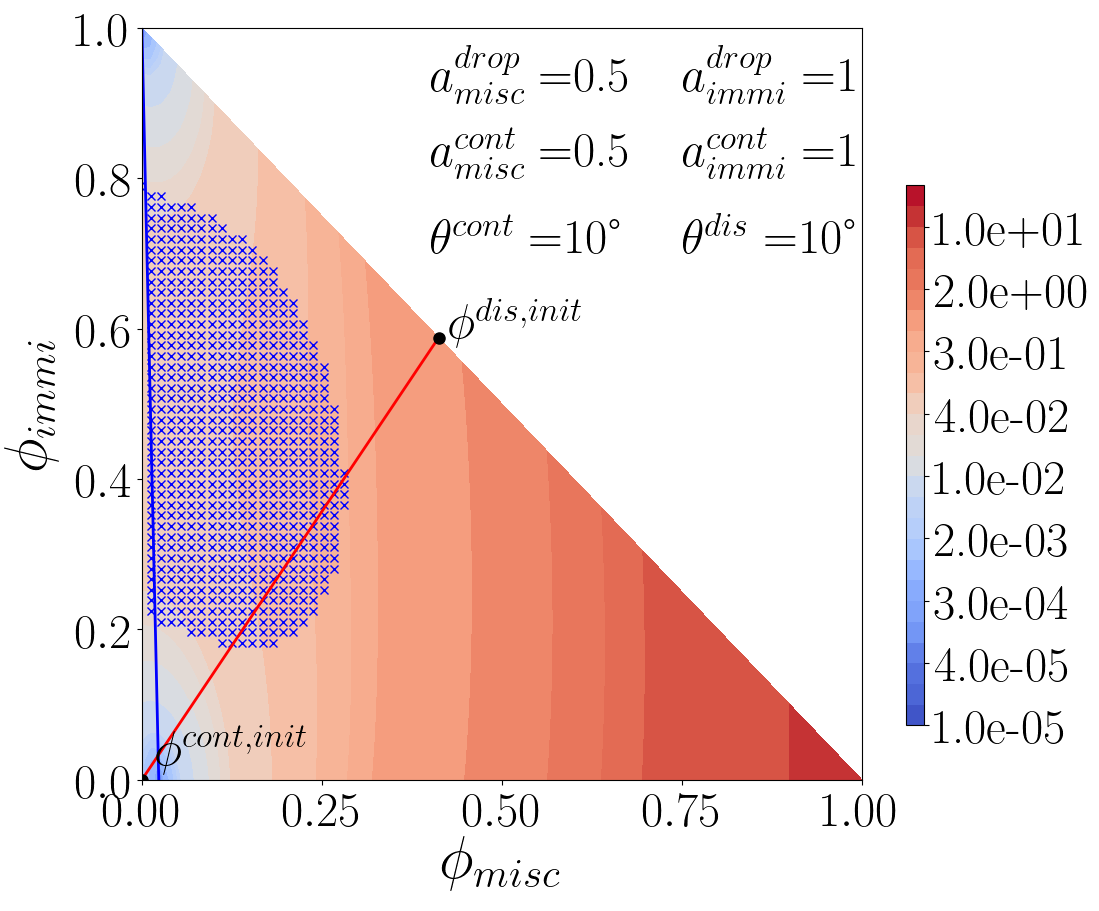
\includegraphics[width=\textwidth]{figure/paysage_neqlocal}
 		\caption{Paysage thermodynamique complet}
 		\label{fig:y equals x}
 	\end{subfigure}
 	\hfill
 	\begin{subfigure}[H]{0.45\textwidth}
 		\centering
 		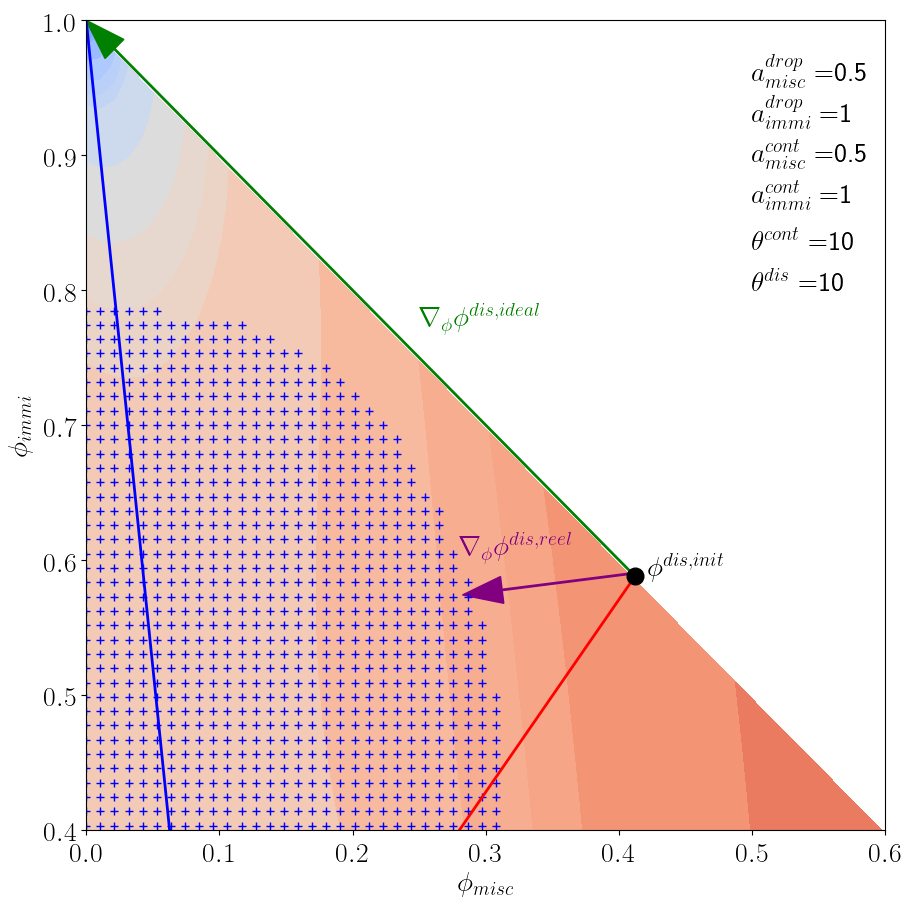
\includegraphics[width=\textwidth]{figure/direction_gradient}
 		\caption{Paysage thermodynamique partiel}
 		\label{fig:gradpasbon}
 	\end{subfigure}
 	\caption{Paysage thermodynamique et direction privilégiée par le système, la flèche verte représente le cas idéal sans intrusion d'eau et la flèche violette le cas associé au paysage thermodynamique, la zone bleu correspond à la zone instable}
 	\label{fig:paysage2}
 \end{figure}\vspace{-0.9cm}
 \begin{figure}[H]
 	\centering
 	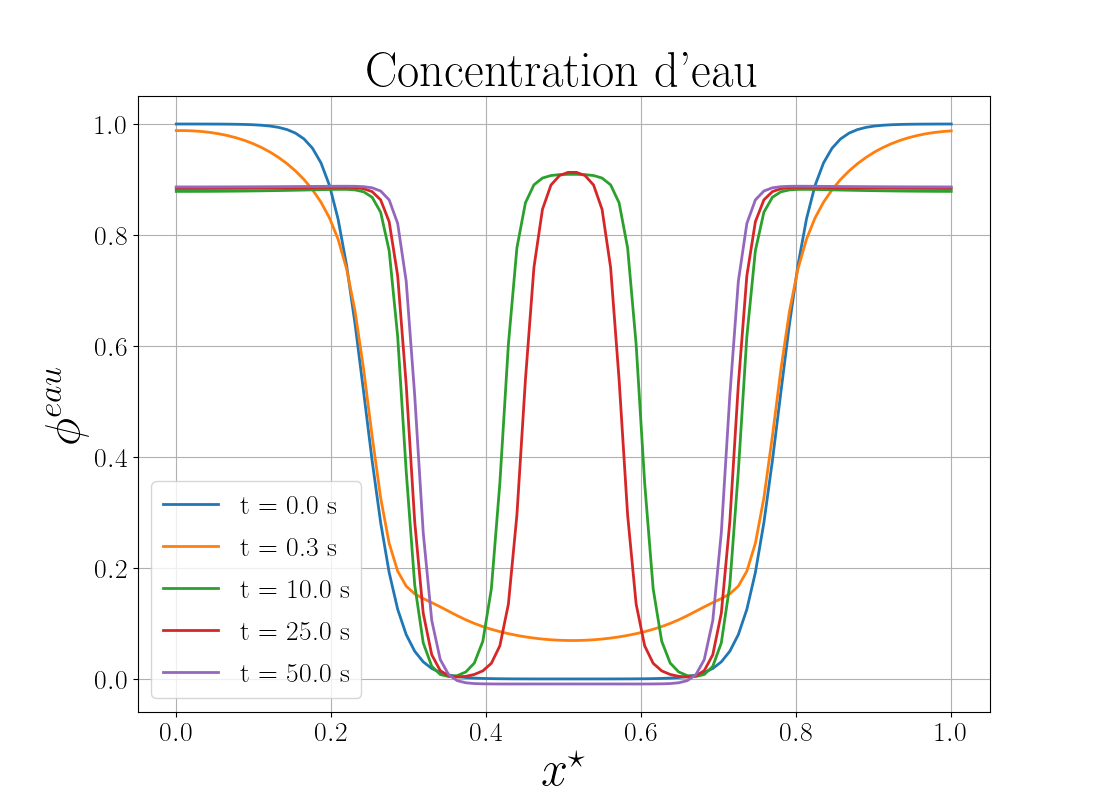
\includegraphics[width=0.5\linewidth]{figure/eau_ref}
 	\caption[Concentration d'eau dans le domaine]{Concentration d'eau dans le domaine, $x^{\star} = x / L_x$ représente une longueur adimensionnée}
 	\label{fig:eauref}
 \end{figure}\vspace{-0.7cm}
Finalement au travers de ces deux exemples, nous avons montré que la représentation graphique pouvait fournir certaines informations sur le comportement du système. Les critères concerne la position des conditions initiales, qui doivent être en dehors de la zone instable, un second critère concerne l'absence nécessaire de la zone instable sur le "chemin" de chacune des phases et finalement une direction initiale privilégiant une imperméabilité à l'eau dans la goutte.
\section{Simulations statiques}
Une fois les critères graphiques validés, l'objectif est de savoir si le paysage transcrit un comportement cohérent du système, pour cela on présente, en figure \ref{fig:thechoosenone} un paysage thermodynamique qui répond à tous les critères soumis précédemment.
\begin{figure}[H]
		\centering
		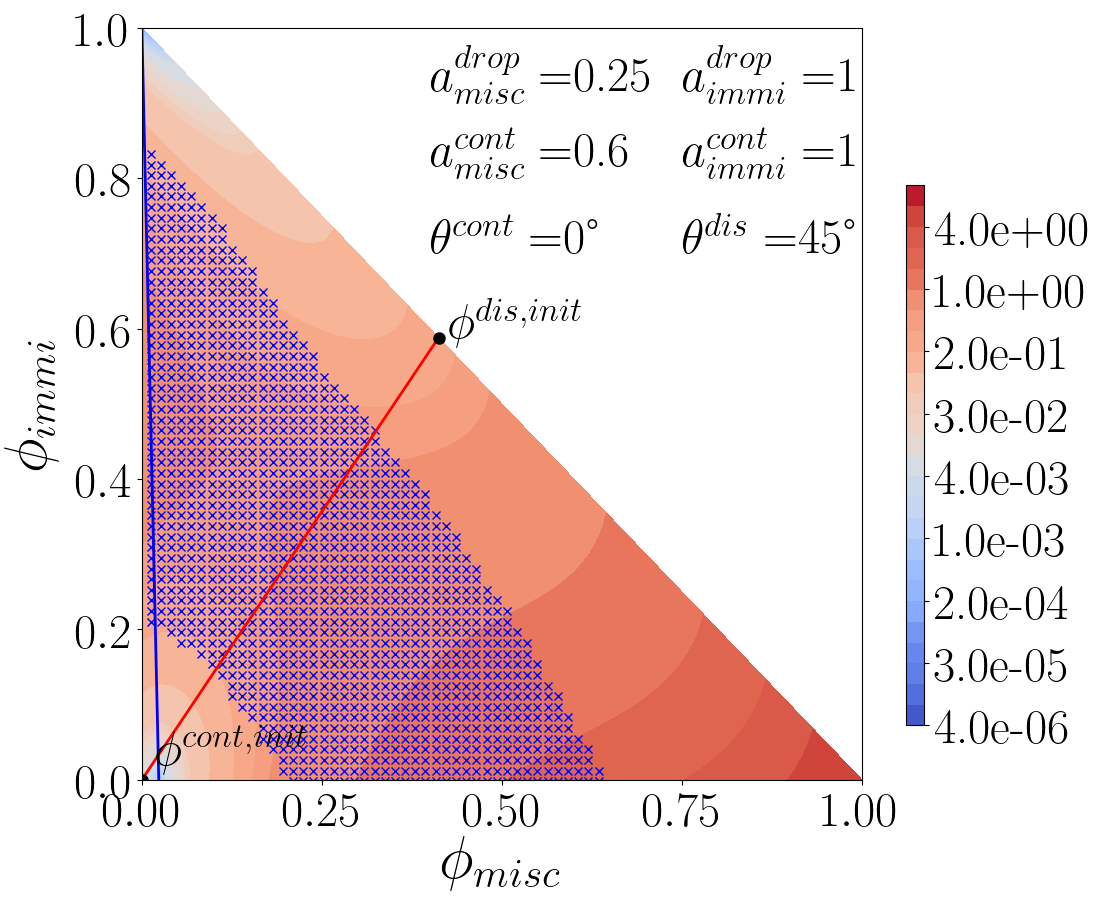
\includegraphics[width=0.45\textwidth]{figure/Paysage_ecriture1.png}
	\caption{Paysage thermodynamique choisit pour la simulation}
	\label{fig:thechoosenone}
\end{figure}

Pour démontrer la consistance de ce paysage on réalise une simulation statique, sans couplage avec les équations de Navier-Stokes. La figure \ref{fig:resultstatiquegoodlandscape} présente les résultats, on observe une non-monotonie de l'interface pour le composant miscible en régime stationnaire, de plus à l'intérieur de la goutte la concentration de composant miscible est négative et la composition d'élément immiscible est quant à elle supérieure à 1, de façon à obtenir une somme des deux concentrations égale à l'unité. Il est cependant possible d'observer que ce paysage préserve la goutte d'intrusion d'eau.
\begin{figure}[H]
	\centering
	\begin{subfigure}[H]{0.45\textwidth}
		\centering
		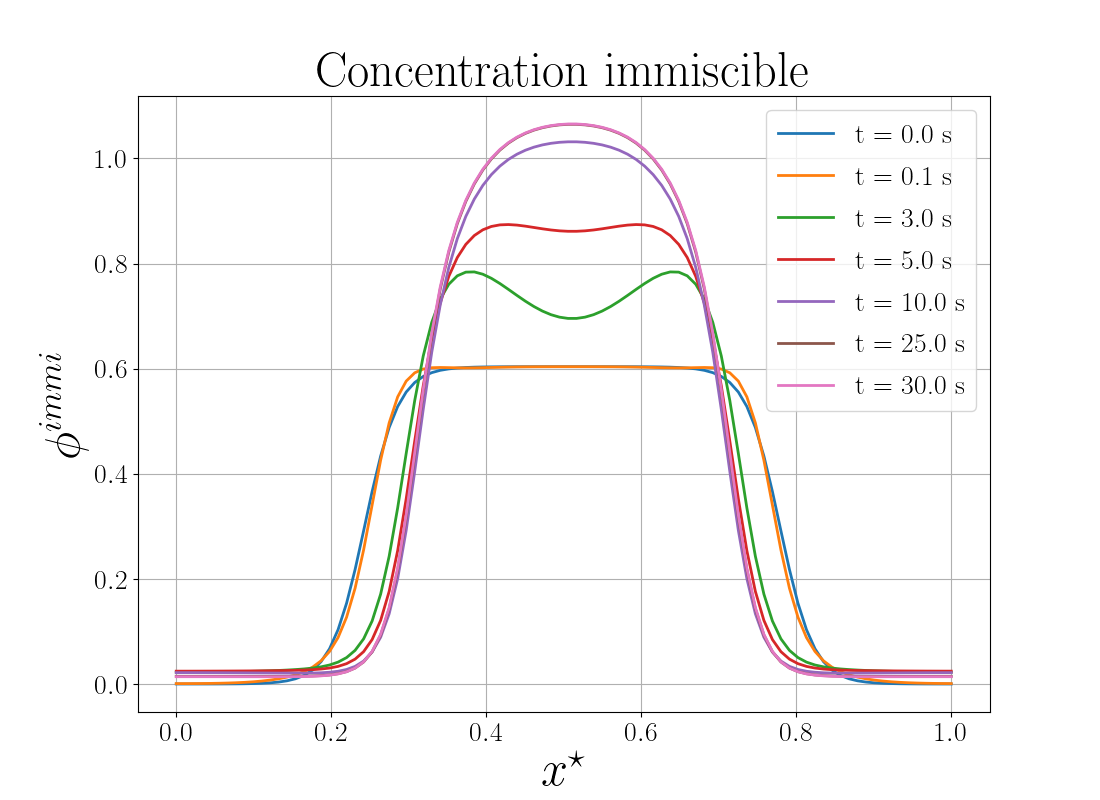
\includegraphics[width=\textwidth]{figure/nouveau_parametrage/immiscible_New_Parametrage.png}
		\caption{Concentration immiscible}
		\label{fig:y equals x}
	\end{subfigure}
	\hfill
	\begin{subfigure}[H]{0.45\textwidth}
		\centering
		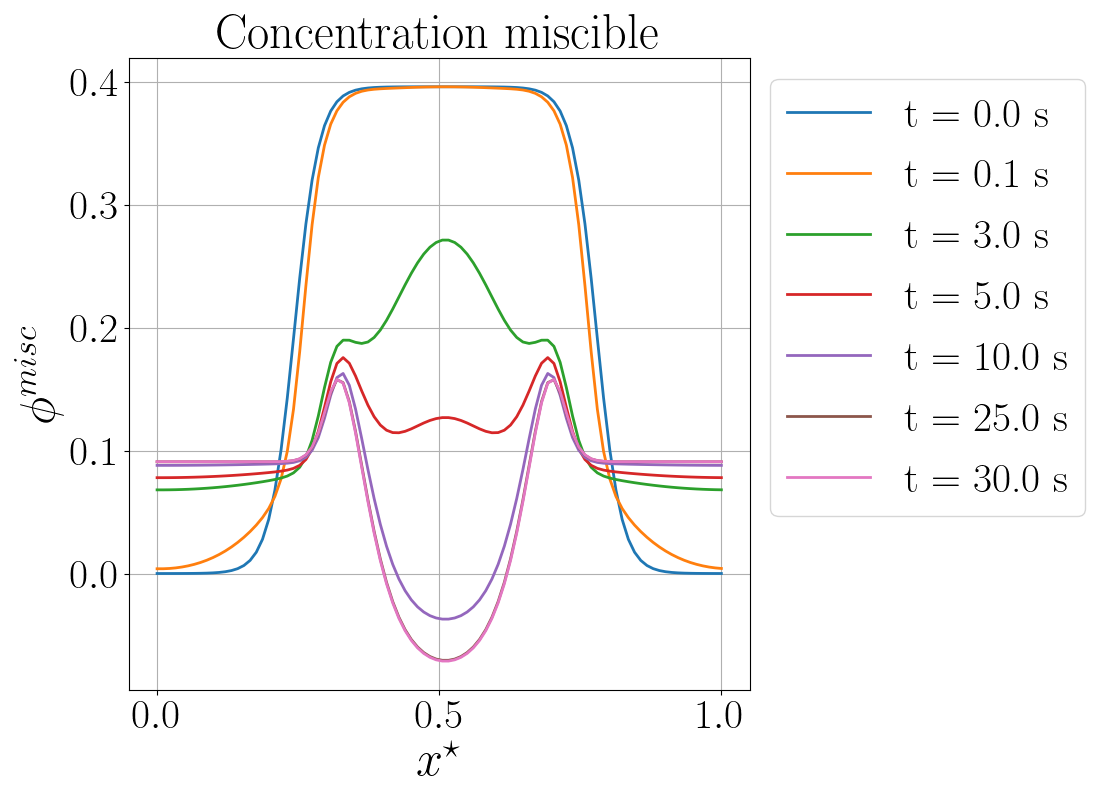
\includegraphics[width=\textwidth]{figure/nouveau_parametrage/miscible_New_Parametrage.png}
		\caption{Concentration miscible}
		\label{fig:y equals x}
	\end{subfigure}
\end{figure} \vspace{-0.8cm}
\begin{figure}[H]
	\centering
	\ContinuedFloat
	\begin{subfigure}[H]{0.45\textwidth}
		\centering
		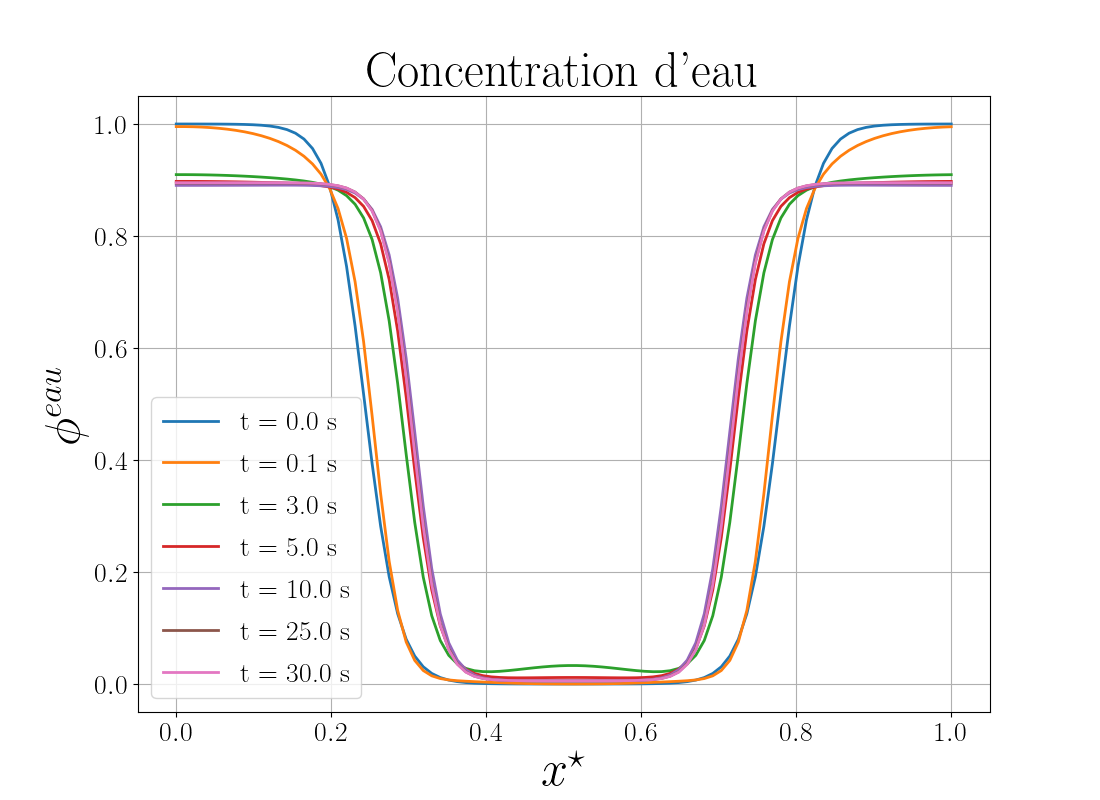
\includegraphics[width=\textwidth]{figure/nouveau_parametrage/eau_New_Parametrage.png}
		\caption{Concentration d'eau}
	\end{subfigure}
	\caption{Variation de la concentration des différents composants au cours du temps}
	\label{fig:resultstatiquegoodlandscape}
\end{figure}
Comme expliqué au chapitre \ref{chap:2} le coefficient de gradient a un impact direct sur le profil d'interface, l'article \cite{rasolofomanana_diffuse-interface_2022} présente un paramétrisation du coefficient de gradient pour traiter les non monotonie d'interface.
Cette dernière a été développé pour étudier les perturbations liées à la différence de position des interfaces. En effet les interfaces étant suivi implicitement, chaque composant possède une interface qui lui est propre, la différence de position entraîne alors un excès de masse ainsi qu'une non monotonie sur le profil d'interface. Cette non monotonie peut alors être source d'apparition  d'instabilité de Rayleigh Taylor purement numérique, résultant de changements de densité non monotone. Cette paramétrisation utilise la symétrie de la matrice coefficient de gradient pour la réécrire sous la forme :
\begin{equation}
\bar{\bar{\bm{\kappa}}} = \alpha \bm{R}\bm{D}\bm{R}^T
\label{eq:param_kappa}
\end{equation}
avec : $\bm{R}$ une matrice de rotation et $\bm{D}$ une matrice diagonale de la forme :
\begin{equation}
\bm{R} =    \begin{pmatrix} 
\cos\varphi & -\sin\varphi \\ 
\sin\varphi				&  \cos\varphi
\end{pmatrix}
\end{equation}
\begin{equation}
	\bm{D}(d) =    \begin{pmatrix} 
	2 & 0 \\ 
	0 & d
	\end{pmatrix} 
\end{equation}
La cohérence avec le système binaire est assurée par le coefficient $\alpha$ obtenu tel que :
\begin{equation}
\alpha = \frac{\kappa^{bin}}{2\cos^2\varphi + d \sin^2\varphi}
\end{equation}
Les résultats de la paramétrisation de l'interface sont présentés en figure \ref{fig:profinterfacekappa}, on y observe effectivement un impact du choix de la matrice de coefficient de gradient sur le profil d'interface en régime stationnaire, cependant on remarque également qu'il est difficilement imaginable de complètement "lissé" notre interface à l'aide de cette méthode. De plus il est possible d'observer que la réduction de la non-monotonie s'accompagne d'un élargissement important de l'interface.
\begin{figure}[H]
		\centering
		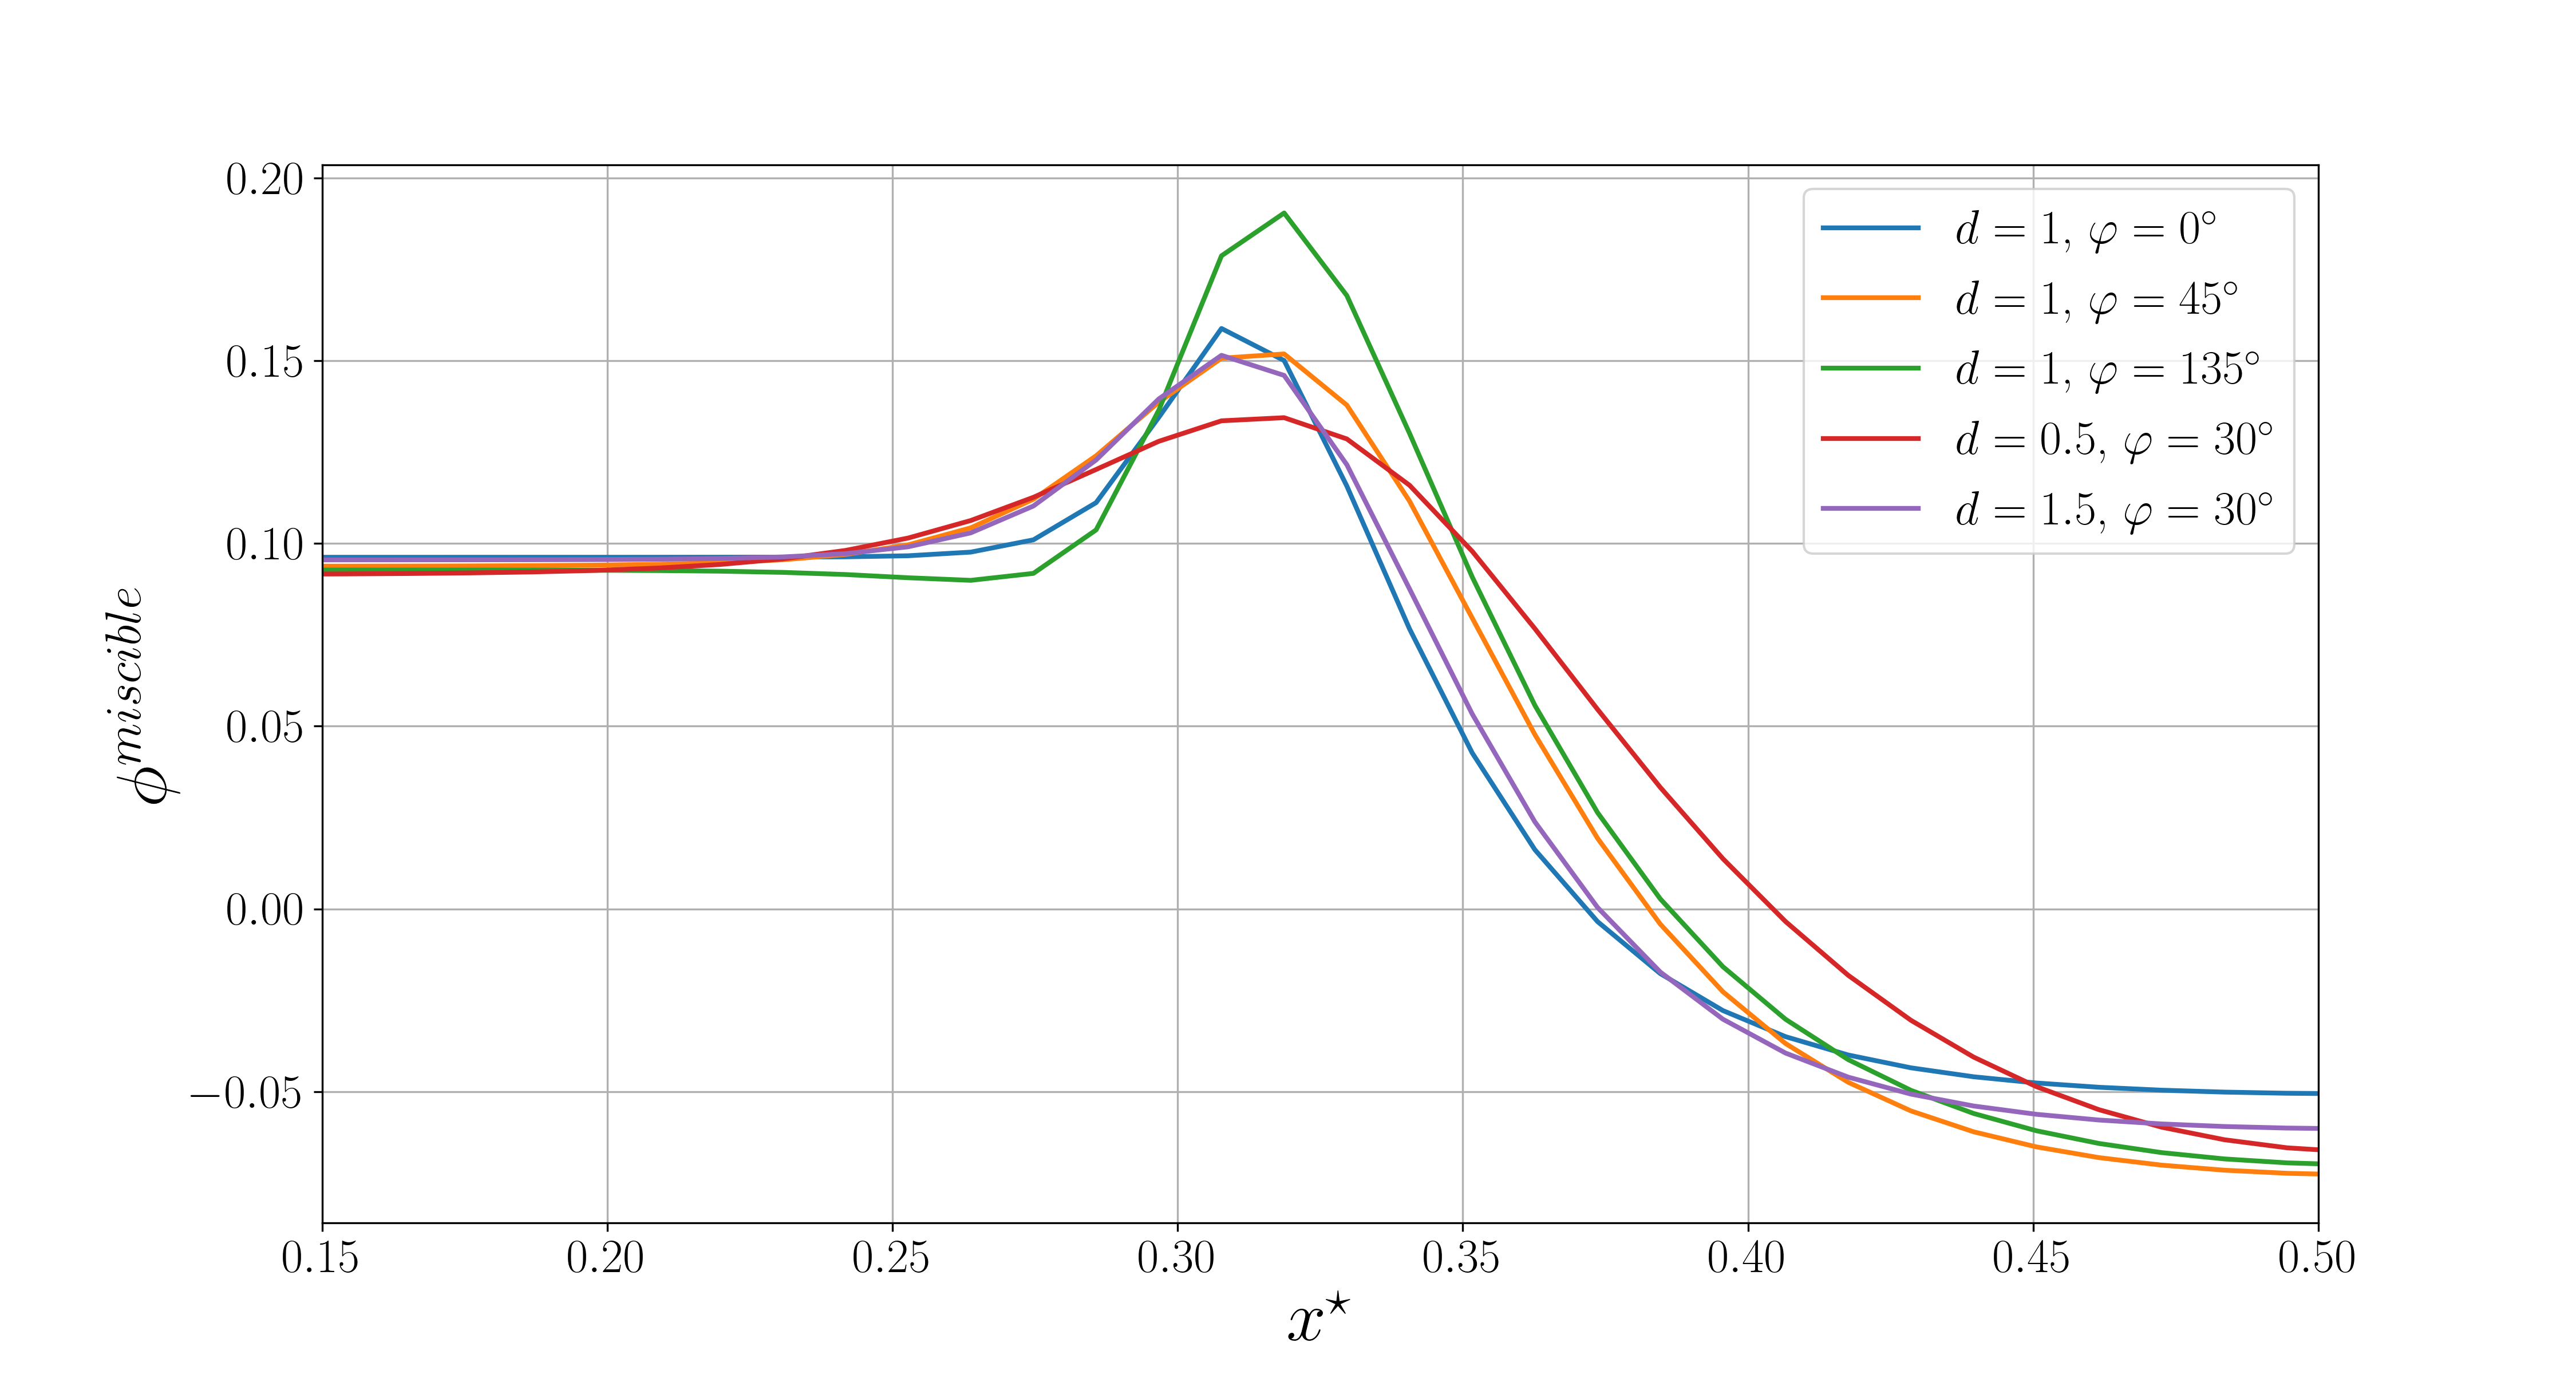
\includegraphics[width=0.7\textwidth]{figure/ProfInterfStatio2.png}
		\caption{Profils de l'interface pour différents paramétrages du coefficient de gradient}
		\label{fig:profinterfacekappa}
\end{figure}

